% CAPITOLO 2 — STORYBOARDS
\chapter{Storyboards}
\label{cap:storyboards}

\section{Autenticazione e Area Personale}

\subsection{Autenticati}
La schermata di accesso permette all'utente di autenticarsi inserendo le proprie credenziali (email e password).
\begin{figure}[H]
    \centering
    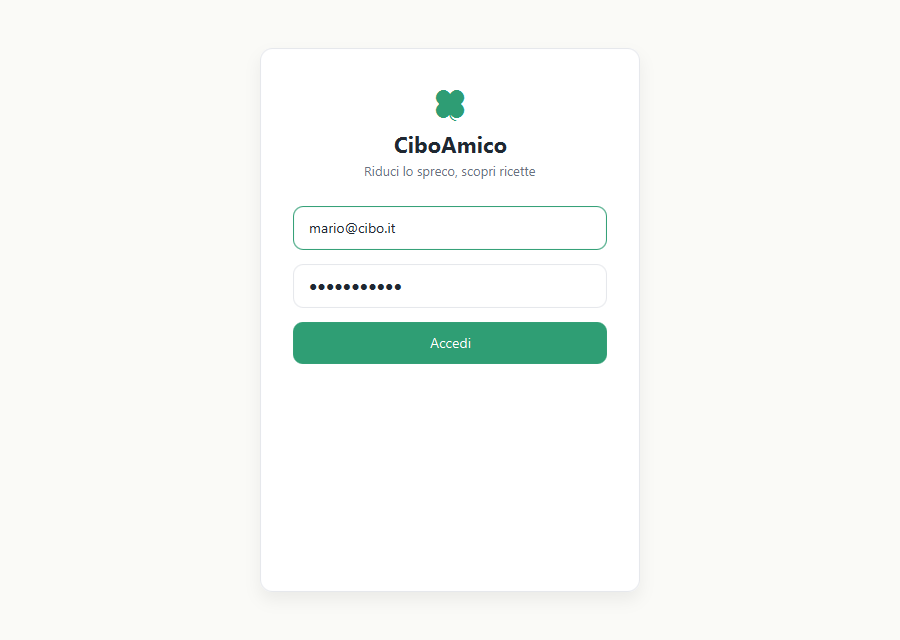
\includegraphics[width=0.8\textwidth]{figures/schermata-login.png}
    \caption{Schermata di autenticazione al sistema.}
    \label{fig:sb_login}
\end{figure}

\subsection{Home (Cliente)}
Completata l'autenticazione, il Cliente raggiunge la dashboard principale, dalla quale accede alle aree del sistema.
\begin{figure}[H]
    \centering
    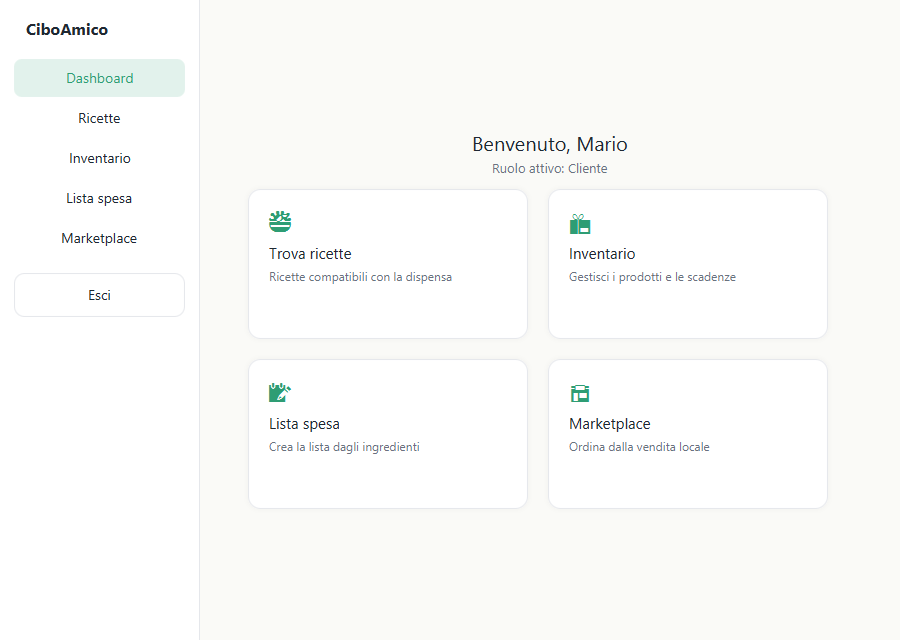
\includegraphics[width=0.8\textwidth]{figures/schermata-home.png}
    \caption{Dashboard principale lato Cliente.}
    \label{fig:sb_home}
\end{figure}

\section{Gestione Domestica}

\subsection{Gestisci Dispensa}
L'interfaccia di gestione dell'inventario mostra gli alimenti della dispensa con quantità e date di scadenza, evidenziando i prodotti prossimi alla scadenza.
\begin{figure}[H]
    \centering
    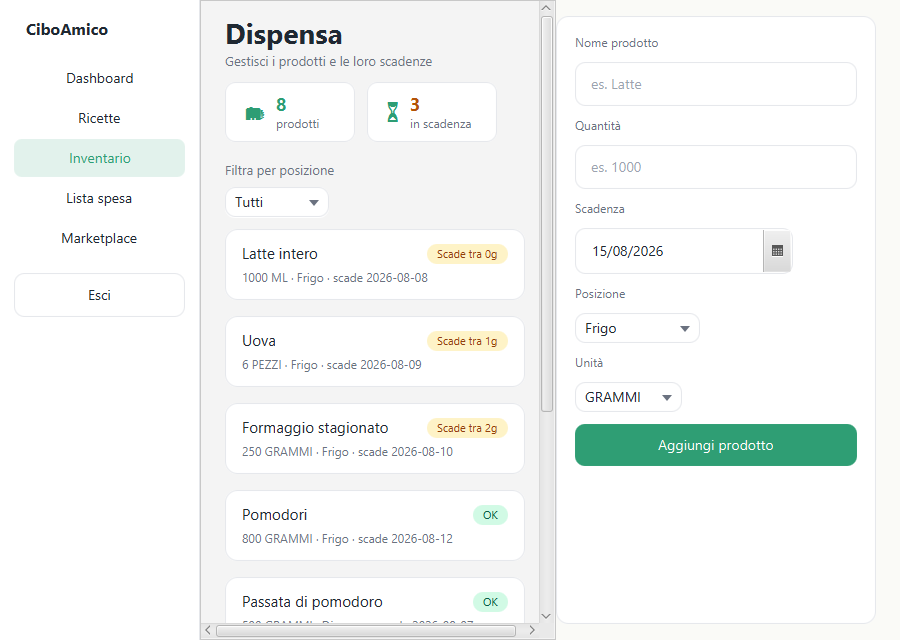
\includegraphics[width=0.8\textwidth]{figures/schermata-inventario.png}
    \caption{Interfaccia per il monitoraggio della dispensa e delle scadenze.}
    \label{fig:sb_inventario}
\end{figure}

\subsection{Trova Ricette Compatibili}
L'utente visualizza le ricette suggerite in base agli ingredienti disponibili in dispensa, con l'elenco degli ingredienti di ciascuna.
\begin{figure}[H]
    \centering
    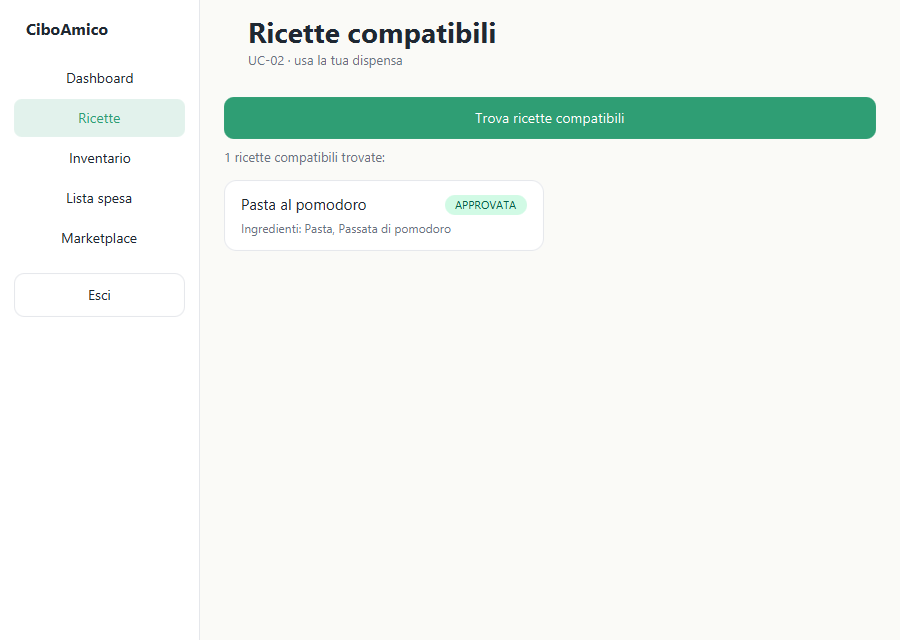
\includegraphics[width=0.8\textwidth]{figures/schermata-ricette.png}
    \caption{Schermata dei suggerimenti per le ricette compatibili.}
    \label{fig:sb_ricette}
\end{figure}

\section{Acquisti e Marketplace}

\subsection{Calcola Lista della Spesa}
Il sistema determina gli ingredienti mancanti per una ricetta selezionata, restituendo la lista della spesa precisa.
\begin{figure}[H]
    \centering
    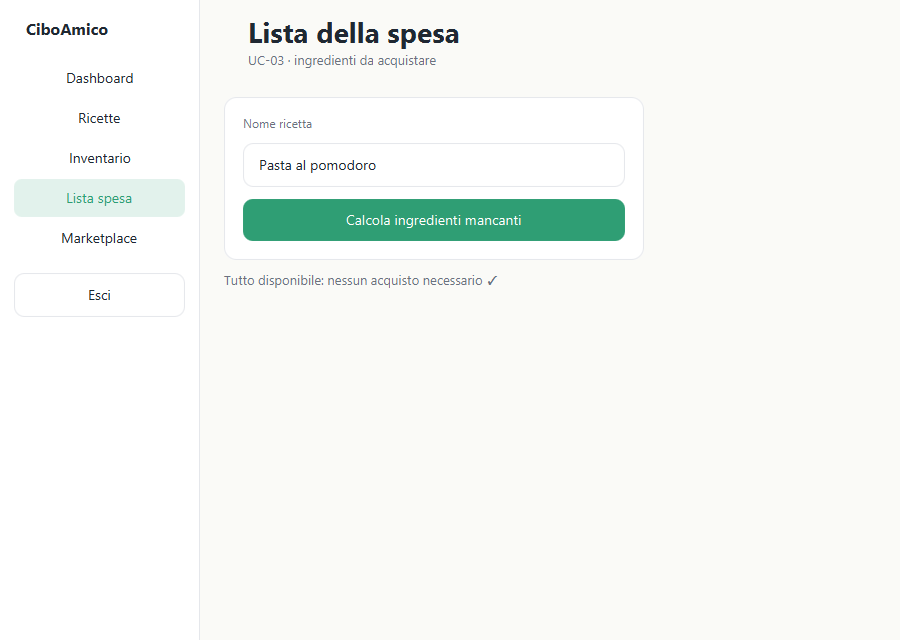
\includegraphics[width=0.8\textwidth]{figures/schermata-lista-spesa.png}
    \caption{Lista della spesa calcolata a partire dagli ingredienti mancanti.}
    \label{fig:sb_lista}
\end{figure}

\subsection{Marketplace (Ricerca Prodotti)}
L'area dedicata all'acquisto diretto mostra i prodotti locali dei venditori, con prezzo e disponibilità residua.
\begin{figure}[H]
    \centering
    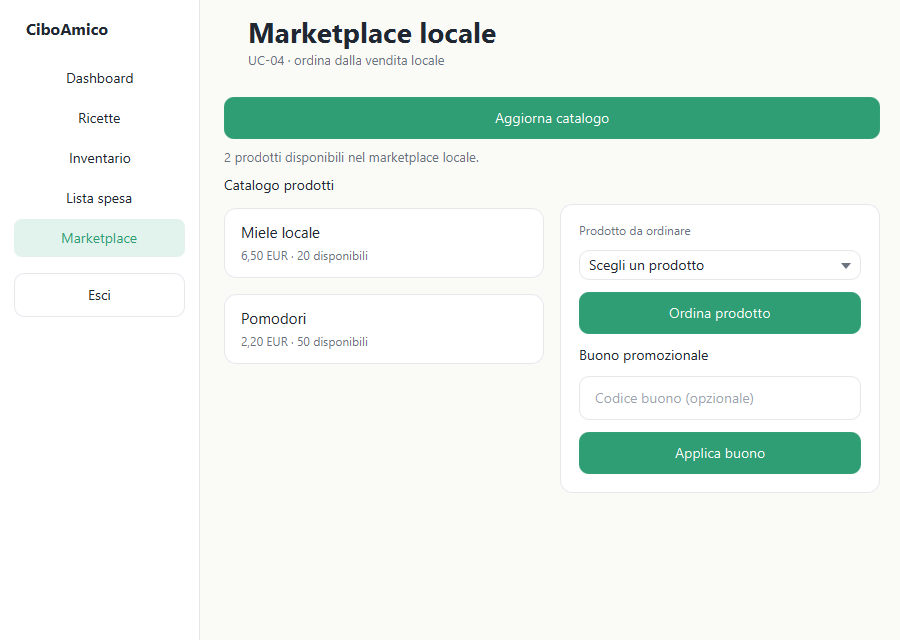
\includegraphics[width=0.8\textwidth]{figures/schermata-marketplace.png}
    \caption{Catalogo dei prodotti locali disponibili per l'acquisto.}
    \label{fig:sb_marketplace}
\end{figure}

\subsection{Ordina un Prodotto}
Il sistema presenta il riepilogo dell'ordine selezionato e consente di procedere con l'acquisto.
\begin{figure}[H]
    \centering
    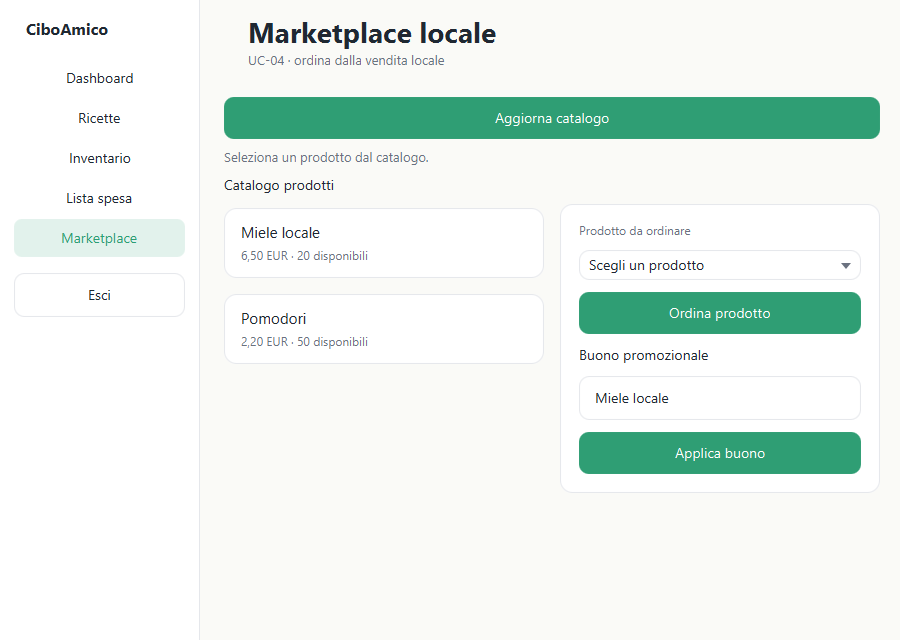
\includegraphics[width=0.8\textwidth]{figures/schermata-ordine.png}
    \caption{Schermata dell'ordine e del riepilogo.}
    \label{fig:sb_ordine}
\end{figure}

\subsection{Ordina un Prodotto con Buono Promozionale}
L'interfaccia consente di inserire un codice di buono promozionale: il sistema valida il buono e ricalcola il totale applicando lo sconto (estensione del caso d'uso \emph{Ordina un Prodotto}).
\begin{figure}[H]
    \centering
    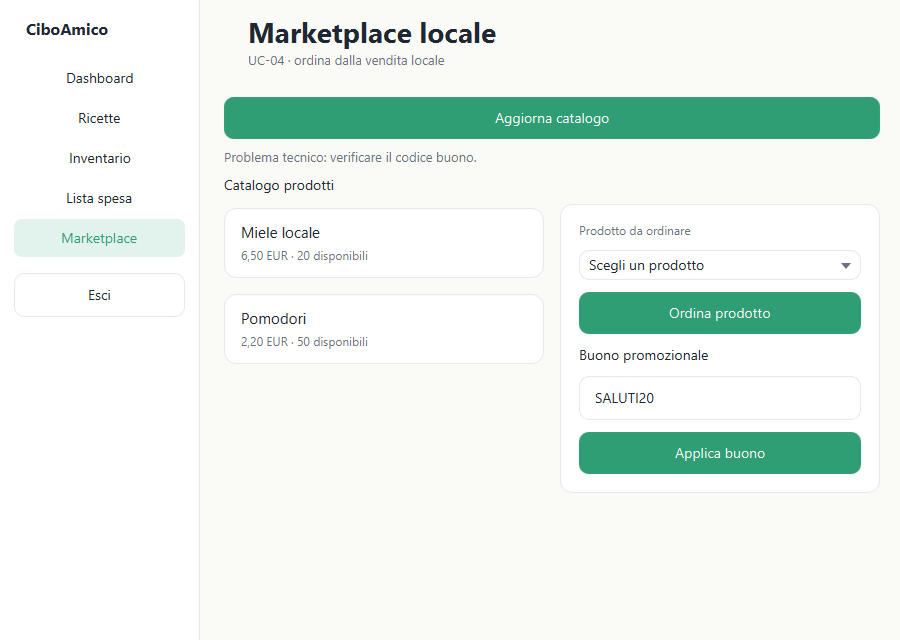
\includegraphics[width=0.8\textwidth]{figures/schermata-ordine-buono.png}
    \caption{Applicazione di un buono promozionale e totale scontato.}
    \label{fig:sb_buono}
\end{figure}

\subsection{Pagamento (passo 6)}
Confermato l'ordine, l'interfaccia passa alla schermata di pagamento: l'utente inserisce i dati della carta (numero, intestatario, scadenza e CVV) e autorizza l'addebito; l'esito è mostrato inline nella stessa vista, come richiesto dall'estensione \textbf{6a} (pagamento rifiutato) del caso d'uso.
\begin{figure}[H]
    \centering
    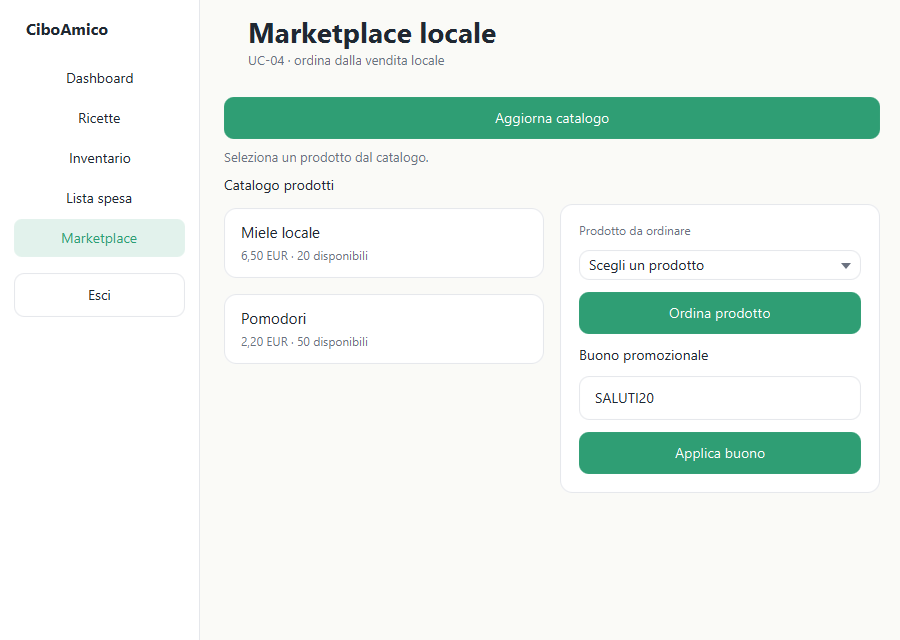
\includegraphics[width=0.8\textwidth]{figures/schermata-payment.png}
    \caption{Schermata di pagamento (dati carta e autorizzazione all'addebito).}
    \label{fig:sb_payment}
\end{figure}

\section{Area Amministratore}

\subsection{Approvazioni venditori e ricette}
L'Amministratore gestisce le richieste di approvazione: la vista mostra i venditori e le ricette in attesa di validazione e consente di approvarle o rifiutarle. L'area amministrativa è separata da quella del Cliente, come da modello dei casi d'uso.
\begin{figure}[H]
    \centering
    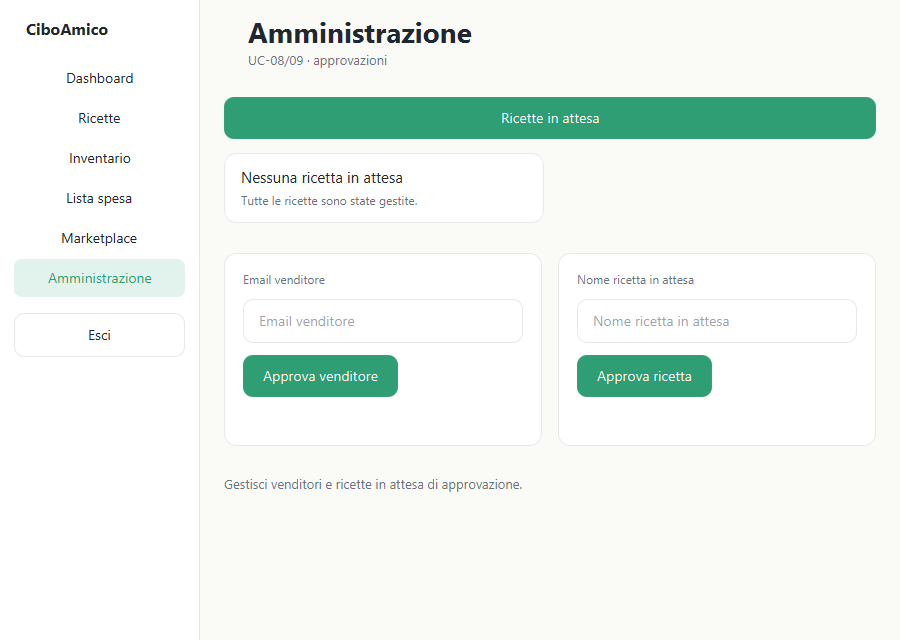
\includegraphics[width=0.8\textwidth]{figures/schermata-admin-approvazioni.png}
    \caption{Vista amministratore per le approvazioni di venditori e ricette.}
    \label{fig:sb_admin}
\end{figure}
